Levando em consideração $V_a$ como a tensão aplicada no enrolamento, $I_a$ como a corrente no enrolamento e $e_a$ como a tensão induzida no enrolamento. 

\begin{figure}[ht!]
    \center 
    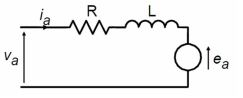
\includegraphics[scale=1]{imagens/f22}
    \caption{Modelo do Motor de Passo}
\end{figure}

No enrolamento A do motor:

$$V_a=Ri_a+L\frac{di_a}{dt}+e_a$$

No enrolamento B do motor: 

$$V_b=Ri_b+L\frac{di_b}{dt}+e_b$$

Para os fluxos magnéticos $\Psi_a$ no enrolamento A, $\Psi_b$ no enrolamento B e  $\Psi_m$ sendo o fluxo máximo no estator, tem-se que: 

$$\Psi_a=\Psi_m \cos (n\theta)$$
$$\Psi_b=\Psi_m \sin (n\theta) $$

As tensões induzidas nos enrolamentos do estator $e_a$ e $e_b$, considerando o número de espiras no enrolamento do estator "m", são dadas por: 

$$e_a=m\frac{d\Psi_a}{dt}=-mn\Psi_m\sin(n\theta)\frac{d\theta}{dt}= -k_c\omega \sin(n\theta)$$
$$e_b=m\frac{d\Psi_b}{dt}=-mn\Psi_m\cos(n\theta)\frac{d\theta}{dt}= k_c\omega \cos(n\theta)$$

Utilizando a conservação de energia onde a potência mecânica na saída é igual à potência elétrica na entrada, tem-se: 

$$\omega T_a=i_a e_a $$ 
$$\omega T_b=i_b e_b$$

Portanto: 

$$T_a=-i_aK_c\sin(n\theta)$$
$$T_b=i_bK_c\cos(n\theta)$$

Juntando as equações, podemos chegar no modelo completo do motor de passo: 

$$J_r\frac{d^2\theta}{dt^2}+D_r\frac{d\theta}{dt}= T+T_a+T_b=T-i_aK_c\sin(n\theta)+i_bK_c\cos(n\theta)$$
$$V_a=Ri_a+L\frac{di_a}{dt}-\omega K_c\sin(n\theta)$$
$$V_b=Ri_b+L\frac{di_b}{dt}+\omega K_c\cos(n\theta)$$

